\documentclass[letterpaper]{article}

\usepackage{natbib,alifexi}
\usepackage{amsmath}
\usepackage[french]{babel}
\usepackage[utf8]{inputenc}
\usepackage{hyperref}
\usepackage{amsfonts}
\usepackage{graphicx}
\usepackage{blkarray}
\usepackage{tikz}
\usetikzlibrary{automata, positioning}

\newcommand{\colornode}[1][]{\node[state,
	    align=center,
	    text=gray!40!black,
	    draw=gray,
	    fill=gray!20!white,{#1}]}
\newcommand{\bigcolornode}[1][]{\node[state,
	    align=center,
	    text=gray!40!black,
	    draw=gray,
	    fill=gray!20!white,
	    text width=1.7cm,{#1}]}

\newcommand{\drawedge}{\draw[every loop, line width=0.4mm, fill=gray, draw=gray]}

\newcommand*{\fullref}[1]{\hyperref[{#1}]{\autoref*{#1} \nameref*{#1}}}


\title{Etude du Monopoly via les chaînes de Markov}
\author{Rémy Detobel\\
\mbox{}\\
Université Libre de Bruxelles, Bruxelles, Belgique \\
rdetobel@ulb.ac.be}


\begin{document}
\maketitle

\begin{abstract}
  Etude du Monopoly à travers un modèle simple de processus probabiliste 
  que sont les chaines de Markov.  Les conceptes principaux de ce modèle
  seront présenté et expliqué.  Une adptation de cette chaine sera 
  également effectuée pour correspondre au fonctionnement du Monopoly 
  (un jeu de plateau classique).\\
  Un algorithme a également été créé pour mettre en application les chaines
  de Markov et calculer les terrains les plus rentables, les plus fréquentés.
\end{abstract}

\section{Introduction}
%   \citep{BTW87,BTW88}
  Contrairement aux idées reçues, les cases du Monopoly ne sont pas équiréparties.  Pour
  pouvoir décrire la probabiliter de tombé sur chaque case, on va utiliser les chaînes
  de Markov.  Ce document définira donc les chaines de Markov ainsi que d'autres 
  notions utiles pour résoudre ce problème.  Des choix devront également être fait pour 
  permettre de modéliser ce problème et le rendre totalement compatible avec la structure
  des chaines de Markov.
  % TODO ajouter des informations à l'intro
  
\section{Approche théorique}
  
  \subsection{Les chaines de Markov}
    Une chaîne de Markov est une représentation graphique permettant 
    de modéliser l'état d'un système en se basant uniquement sur l'état précédent. La
    structure utilisée dans ce rapport sera toujours considérée en temps discret.
    Une chaine de Markov est composée de noeud et d'arrête reliant ces noeuds.  Chaque
    noeud représente un état du système tendis qu'une arrête permet d'indiquer les 
    diférents liens entre ces états.  Chaque arrête à un poid représentant la probabilité 
    que ce changement d'état se produise.\\
    \begin{center}
      \begin{tikzpicture}
	% Draw the states
	\colornode (e1) {Etat 1};
	\colornode[right=of e1] (e2) {Etat 2};

	% Connect the states with arrows
        \drawedge
  	  (e1) edge[bend right, auto=right] node {Arrête 1} (e2)
  	  (e2) edge[bend right, auto=right] node {Arrête 2} (e1)
  	  (e2) edge[loop above]             node {Arrête 3} (e2);
      \end{tikzpicture}
    \end{center}
    
    Par définition, la somme des poids des arrêtes partant d'un poid doivent valoir 1.  
    De manière plus formel, les chaînes de Markov sont réprésentées via la formule 
    mathématique suivante:
    $$\mathcal{M} = (S, \mathbf{P}, \iota_{init})$$
    Où $S$ représente l'ensemble de tous les états possible, $P$ une matrice $S \times S$
    où chaque élément est compris entre 0 et 1 et où cette valeur représente la probabilité 
    de passé d'un état à un autre (respectivement, l'état correspondant à la ligne et à la colonne).
    $\iota_{init}$ est une matrice colonne où chaque ligne représente un état et la valeur
    associée représente la probabilité de commencer par cet état.  On peut retrouver d'autres
    variables dans la litérature (comme $AP$ et $L$ par exemple) mais celles-ci ne seront pas 
    utiles dans cet article.\\
    
  \subsection{Probabilité}
    Dans une chaine de Markov, on s'intéresse à la ``probabilité'' de se trouver dans un certain 
    état ou la probabilité de passé d'un état à un autre.  Définir formellement une probabilité
    est un travail long et complexe, il ne sera donc pas fait dans ce document.  Cependant, 
    on peut se représenter une probabilité comme étant la ``chance'' de passer d'un état à un autre.
    Par exemple, si une arrête reliant l'état $s$ à $s'$ à une probabilité de $0.5$, on peut en 
    déduire qu'il y a une ``chance'' sur deux que le système passe de l'état $s$ à $s'$.
    Cette exemple sera noté plus formellement de la manière suivante:
    $$\mathbf{P}(s, s') = 0.5$$
    Où $s$ et $s'$ sont des états et $0.5$ la probabilité de passer du premier état au second 
    état (respectivement donc $s$ et $s'$).\\
    Il n'est pas toujours simple de mesurer une probabilité.  Une technique assez intuitive est 
    de reproduire une expérience (chaque expérience doit être indépendante des précédentes) 
    
  \subsection{Propriété}
    Comme vu précédemment, la somme des poids des arrêtes partant d'un noeud vallent un.
    Soit pour tous $s \in S$:
    $$\sum\limits_{s' \in S} \mathbf{P}(s, s') = 1$$
    Il en va de même pour la somme des éléments de la matrice de distribution initiale:
    $$\sum\limits_{s \in S} \iota_{init}(s) = 1$$
    Pour qu'un état $s'$ soit le successeur d'un état $s$, il faut que 
    $$\mathbf{P}(s, s') > 0$$
    L'idée est équivalente concernant les chemins (arrêtes).
    
  \subsection{Comportement des chaînes des Markov}
    Les chaînes de Markov peuvent avoir différentes caractéristiques en fonction 
    de leurs structures et des valeurs qu'elles contiennent.  
    Nous en distinguerons 3:
    \begin{itemize}
     \item \textbf{Fortement connexe}: un ensemble est fortemment connexe si pour tout
      les noeuds présent dans cet ensemble peuvent être atteint depuis n'importe quel
      autre noeud également présent dans ce même ensemble.  En d'autres mots, on peut dire 
      que dans un ensemble $T$ il existe un chemin entre l'état $s'$ et $s$ tel que 
      $s$ et $s' \in T$
     \item \textbf{Composant fortement connexe}: un ensemble $T$ est un composé fortement
      connexe s'il est le plus grand ensemble fortement connexe d'une chaîne de Markov.  
      Les compostants fortements connexes sont notés ``SCC'' (qui sont les initiales de
      ``Strongly Connected Component'').
     \item \textbf{BSCC}: il s'agit des initiales de ``Bottom Strongly Connected Component''.
      L'ensemble $T$ est un BSCC de la chaîne de Markov $\mathcal{M}$ si $T$ est un SCC et
      qu'aucun état en dehors de $T$ ne peut être atteint.  En d'autres mots, il faut que
      pour tout $s \in T$, $\mathbb{P}(s, T) = 1$.  Cela signifie que toutes les 
      arrêtes partant de $s$ sont dirigés dans l'ensemble $T$.
    \end{itemize}
    Lorsque l'on se trouve dans un état présent dans un BSCC, on ne quitte plus jamais ce
    BSCC, même après une infinité de changement d'état.  On a donc une probabilité 1 de 
    se retrouver dans ce BSCC après une infinité de changement.
  
  \subsection{Distribution stationnaire}
    Lorsque l'on se trouve dans un état étant lui même dans un BSCC, il est impossible de 
    quitter ce BSCC.  La probabilité dans une chaîne de Markov de se retrouver dans un état
    présent dans le BSCC après une infinité de changement d'état est donc de 1.  Cependant
    tous les états présent dans ce BSCC n'ont pas la même probabilité d'être sélectionné.\\
    On estime qu'on se trouve dans une distribution stationnaire lorsqu'un changement d'état
    supplémentaire ne modifie pas les valeurs de probabilité de chaque état.  De manière plus 
    formel, cela signifie qu'il existe un vecteur $v$ où chaque terme est compris entre 0 et 1,
    tel que sa multiplication par la matrice de déplacement donne ce même vecteur.  C'est à dire:
    $$v P = v$$
    Où $v$ est le vecteur décrivant la distribution stationnaire et $P$ la matrice de déplacement.
    
    \subsubsection{Calcul de la distribution stationnaire}
      \label{etat_stationnaire}
      Il existe différentes façon de calculer l'état stationnaire d'une chaine de Markov.
      Plusieurs méthodes sont décrite dans le livre ``Introduction to Probability'' (\citep{IP}) 
      dans le chapitre 11.\\
      On sait que la somme des composants du vecteur $v$ décrivant la distribution stationnaire 
      fait 1.  On peut donc écire:
      $$v_1 + v_2 + ... + v_n = 1$$
      Où $n$ est le nombre d'élément dans ce vecteur $v$.  On sait que multiplier ce vecteur $v$
      avec le matrice de déplacement ne change pas les valeurs de ce vecteur.  On se retrouve donc
      avec une multplication de matrice qui peut-être subdivisé en $n$ sous calcul (où $n$ est 
      toujours le nombre d'élément dans ce vecteur $v$); plus l'équation décrite ci-dessus.  On a 
      donc $n+1$ équation pour $n$ inconnue.  Le problème peut donc être résolu.\\
      Une autre méthode consiste à fixer une des valeurs du vecteur $v$ et de ainsi trouver les 
      autres valeurs du vecteur.  Une fois ces valeurs trouvées, il suffit de diviser tous les 
      termes par la somme de ceux-ci.
  
  \subsection{Cas concret}
    \label{casconcret}
    Afin de rendre tous ces concepts plus concrèts, on va s'intéresser à un exemple décrivant
    l'état d'un avion.
    
    \subsubsection{Contexte}
      Dans cet exemple, on va considérer que l'avion pourra avoir 6 états différents: en vol,
      attérissage, décollage, au sol, controle et hors service.  On va considérer qu'en moyenne
      après 3 vol un avion doit passer au controle.  On remarque également qu'il y a une chance
      sur 10 que l'avion ne passe pas le controle et soit considéré comme hors service.
      
    \subsubsection{Représentation Graphique}
      Voici donc la chaine de Markov décrivant cette situation:
      \begin{center}
	\begin{tikzpicture}
	  % Draw the states
	  \colornode[text width=1.7cm] (vol) {En vol};
	  
	  \colornode[below left=of vol] (att) {Attérissage};
	  \bigcolornode[below right=of vol] (dec) {Décollage};
	  
	  \bigcolornode[below right=of att] (sol) {Au sol};

	  \bigcolornode[below left=of sol] (ctr) {Controle};
	  \colornode[right=of ctr] (hs) {Hors service};

	  % Connect the states with arrows
	  \drawedge
	    (vol) edge[bend right, auto=right] node {1} (att)
	    (dec) edge[bend right, auto=right] node {1} (vol)
	    (sol) edge[bend right, auto=right] node {1} (dec)
	    (att) edge[bend right, auto=right] node {2/3} (sol)
	    (att) edge[bend right, auto=right] node {1/3} (ctr)
	    (ctr) edge[bend right, auto=left] node {9/10} (sol)
	    (ctr) edge[bend right, auto=right] node {1/10} (hs)
	    (hs) edge[loop right] node {1} (hs);
	\end{tikzpicture}
      \end{center}
      
    \subsubsection{Représentation matricielle}
      Une chaine de Markov peut également être vue comme une matrice où chaque ligne et chaque 
      colonne représente un état.  Les valeurs au sein de la matrice représente le passage
      de la ligne (en lien avec cette valeur) et la colonne associée à cette même valeur.
      Avant de faire cela, il faut énoncer les différents état possible:
      $$\begin{pmatrix}
	\text{En vol}\\
	\text{Décollage}\\
	\text{Attérissage}\\
	\text{Au sol}\\
	\text{Controle}\\
	\text{Hors service}\end{pmatrix}$$
      C'est donc l'ordre de cette matrice qui sera utilisé afin de constitué la matrice 
      représentant la chaine de Markov:
      $$
	\begin{blockarray}{ccccccc}
	& \text{Vol} & \text{Dec.} & \text{Att.} & \text{Sol} & \text{Ctr.} & \text{H.S.} \\
	  \begin{block}{c(cccccc)}
	    \text{Vol}  & 0 & 0 & 1 & 0    & 0   & 0    \\
	    \text{Dec.} & 1 & 0 & 0 & 0    & 0   & 0    \\
	    \text{Att.} & 0 & 0 & 0 & 2/3  & 1/3 & 0    \\
	    \text{Sol}  & 0 & 1 & 0 & 0    & 0   & 0    \\
	    \text{Ctr.} & 0 & 0 & 0 & 9/10 & 0   & 1/10 \\
	    \text{H.S.} & 0 & 0 & 0 & 0    & 0   & 1    \\
	  \end{block}
	\end{blockarray}
      $$
      Si on considère que lorsqu'un avion est mis en service il se trouve dans l'état
      ``au sol'', on peut écrire la matrice initiale de la manière suivante:
      $$
	\begin{blockarray}{cc}
	  \begin{block}{c (c)}
	    \text{Vol}  & 0 \\
	    \text{Dec.} & 0 \\
	    \text{Att.} & 0 \\
	    \text{Sol}  & 1 \\
	    \text{Ctr.} & 0 \\
	    \text{H.S.} & 0 \\
	  \end{block}
	\end{blockarray}
      $$
    
    \subsubsection{Caractéristiques}
      La chaine de Markov résultant de cette exemple à plusieurs propriété.  Tout
      d'abord, cette chaine de Markov contient plusieurs sous partie fortement
      connexe comme par exemple l'ensemble: \{en vol, attérissage, décollage,
      au sol\}.  Cette ensemble reste fortemment connexe si l'on ajoute l'état
      ``controle''.  On a donc l'ensemble: \{en vol, attérissage, décollage,
      au sol, controle\} qui en plus d'être fortemment connexe est un SCC.
      Cette chaine contient également un BSCC formé uniquement de l'état 
      ``Hors Service''.\\
      Pour faire en sorte que toute la chaine de Markov soit un BSCC, il suffirait
      par exemple de permettre à l'état ``Hors service'' de rejoindre à nouveau l'état
      ``controle''.  On pourrait par exemple imaginer qu'il y a une chance sur 100 qu'un
      avion hors service soit repris au controle et soit de nouveau utilisable.
      
\section{Modélisation}

  \subsection{Plateau de jeux}
    Les plateaux de jeux peuvent être vu comme des chaines de Markov.  En effet, on peut 
    voir la position d'un point comme l'état d'un système.  Dans ce type de jeu (comme 
    par exemple le jeu de l'oie) la position du pion dépendra seulement de la case où il 
    se trouvait précédemment et du nombre de case qu'il doit parcourrir (dû par exemple 
    au lancement d'un dé ou à l'indication présente sur la case où le pion se trouvait).
    Les jeux de plateau où le déplacement des pionts n'influancent pas directement la 
    victoire d'un joueur et où chaque case du plateau de jeu peut être visité tout 
    au long de la partie, peuvent être vu comme des BSCC.  
  
  \subsection{Modélisation}
    Le Monopoly peut en effet être vu comme une chaine de Markov.  En effet, comme décrit
    ci-dessus, on peut voir la position d'un point comme l'état d'un système.  Plus 
    concrètement, chaque case sera numérotée et représentera un état de la chaine de Markov.
    \begin{figure}[h]
      \centering
      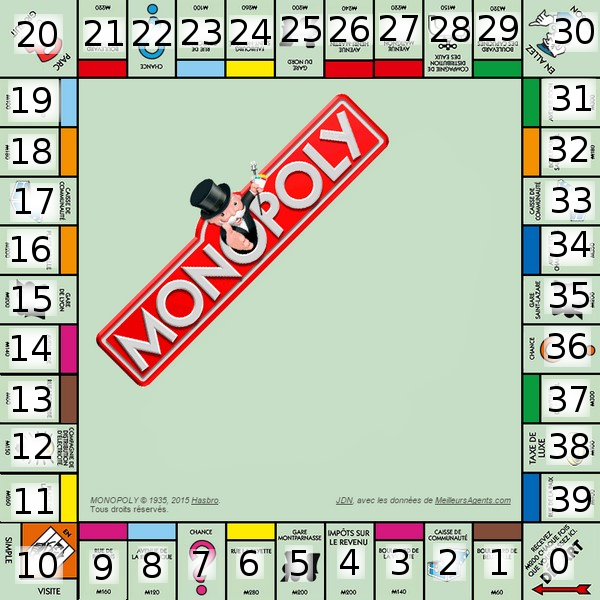
\includegraphics[scale=0.4]{./Images/Monopoly.png}
	\caption{Numéroation du Monopoly \citep{IMG_Monopoly}}
    \end{figure}
    
    Chaque déplacement du piont (c'est-à-dire à chaque fois que l'on lance le dé) sera 
    traduit par un changement d'état.
    Dans un premier temps, on modélise donc le Monopoly par 40 cases où chaque case est
    relié aux $6*n-(n-1)$ cases suivantes, où $n$ est le nombre de dé.  Dans le cas précis
    des règles du Monopoly, chaque case pourra donc accéder à 11 autres cases.  En effet,
    le résultat le plus petit pouvant être produit par $n$ dés est de $n$ (tous les dé à 1).
    On devra donc élminer toutes les $n-1$ cases juste après la case actuelle et le résultat
    le plus grand pouvant être produit par $n$ dés est de $6*n$ (pour un dé à 6 faces).
    \begin{center}
      \begin{tikzpicture}
        \colornode[text width=1cm] at (0, 0) (c0) {Départ};
        \colornode[text width=0.7cm] at (1.5, 0) (c1) {Case 1};
        \colornode[text width=0.7cm] at (3, 0) (c2) {Case 2};
        \colornode[text width=1cm] at (5.5, 0) (cx) {...};
        \colornode[text width=0.7cm] at (7, 0) (c12) {Case 12};
        
        \drawedge
	  (c0) edge[bend left] node {} (c2)
	  (c0) edge[bend left] node {} (cx)
	  (c0) edge[bend left] node {} (c12)
	  (c1) edge[bend right] node {} (cx)
	  (c1) edge[bend right] node {} (c12);
        
      \end{tikzpicture}
    \end{center}
    Cependant, certaines cases ont un comportement particulier comme
    par exemple la case ``aller en prison'' sur laquelle on ne peut pas rester; en effet,
    celle-ci nous redirige directement dans la prison.  La case ``chance'' et ``caisse de
    communauté'' sont égalements des cas particuliers qui font que le Monopoly n'est pas 
    équiréparti.
    
  \subsection{Répartition des dés}
    \label{repart_des}
    Lorsque l'on lance n dés, la somme des valeurs de chanque dés n'a pas la même probabilité
    d'apparaitre.  En effet, lorsque l'on lance 2 dés, il y a 3 manière différentes de formé
    un 4 (à savoir: $3+1$, $2+2$ et $1+3$) alors qu'il n'y a qu'une seule manière de formé un 
    2 (à savoir: $1+1$), comme illustré par la figure \ref{tableau_repartition_des}.
    \begin{figure}[h]
      \centering
      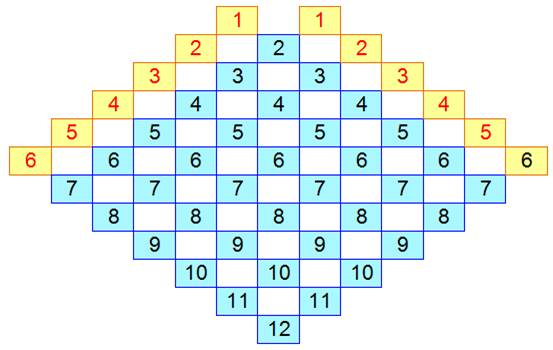
\includegraphics[scale=0.4]{./Images/RepartitionDes.jpg}
	\caption{Répartition des nombres formés avec 2 dés \citep{IMG_Des}}
      \label{tableau_repartition_des}
    \end{figure}
    Cette répartition peut être généralisé de la manière suivante:
    $$\sum\limits_{k=0}^{(s-n)/6} (-1)^k \begin{pmatrix}n \\ k\end{pmatrix} 
      \begin{pmatrix}s-6k-1 \\n-1\end{pmatrix}$$
    Source: %\url{http://villemin.gerard.free.fr/Wwwgvmm/Identite/Identxx2.htm\#formule}\\
    Où $n$ est le nombre de dés et $s$ le nombre que l'on désire former.  Cette equation
    a été construite suite à la décomposition en polynome permettant de calculer des
    réparition.\\
    En effet, en prennant par exemple le polynome $3x + 5x^2 + x^3$ et en le mettant au 
    carré, on va récupérer toutes les combinaissons possibles:
    \begin{align*}
     &(3x \times 3x) + (3x \times 5x^2) + (3x \times x^3) +\\
     &(5x^2 \times 5x^2) + (5x^2 \times x^3) + (x^3 \times x^3)\\
     &= (9x^2) + (15x^3) + (3x^4) + (25x^4) + (5x^5) + (x^6)\\
     &= x^6 + 5x^5 + 28x^4 + 15x^3 + 9x^2
    \end{align*}
    Ce calcul montre la répartition de dés truqués ayant 3 faces 1, 5 faces 2 et une face 3.
    Le résultat final nous montre que lorsque l'on lance 2 de ces dés de 9 faces. En faisant
    la somme des coefficients, on obtient le nombre d'arrangement possible.  Dans le cas
    présent, on a donc $1 + 5 + 28 + 15 + 9$ c'est à dire $59$.  Cela nous permet de dire
    qu'il y a une chance sur 59 que la somme de ses 2 dés forme un 6 et 28 chance sur 59
    de former un 4.\\
    L'équation exprimé au début de ce point représente simplement le développement de 
    ce polynome.
    
  \subsection{Faire un double}
    % TODO un nombre indéfinit de dés... toujours un double où tous les dés les mêmes ?
    Les règles du Monopoly stipulent que lorsque l'on fait 3 doubles à la suite, on est
    envoyé en prison.  Pour modéliser ce comportement via une chaine de Markov, il va 
    falloir triplé le nombre d'état.  En effet, une case $i$ peut être visité après avoir
    fait 0 double, 1 double ou 2 double.  Si de cette case $i$ on refaire encore un double,
    on se retrouve en case prison.  Si par contre on fait un simple nombre, on se retrouve
    de nouveau sur la case $i$ ``zero double''.  Il est assez simple de se rendre compte de
    ça via la figure \ref{representation_double}.  Sur cette image, on peut donc voir en 
    rouge les déplacements fait grace à des doubles.  Ces 3 lignes rouges montre
    donc le déplacement d'un joueur qui aurait lancé les dés et fait consécutivement 3 doubles,
    à savoir ici: $1+1$, $2+2$ et $6+6$.  Ce dernière double le conduit directement en prison.
    Les flèches bleus montrent ce qu'il se passe lorsque l'on fait un simple déplacement (pas un double).
    Elles vont toutes vers la même plateau (celui où on a encore fait zero double).
    \begin{figure}[h]
      \centering
      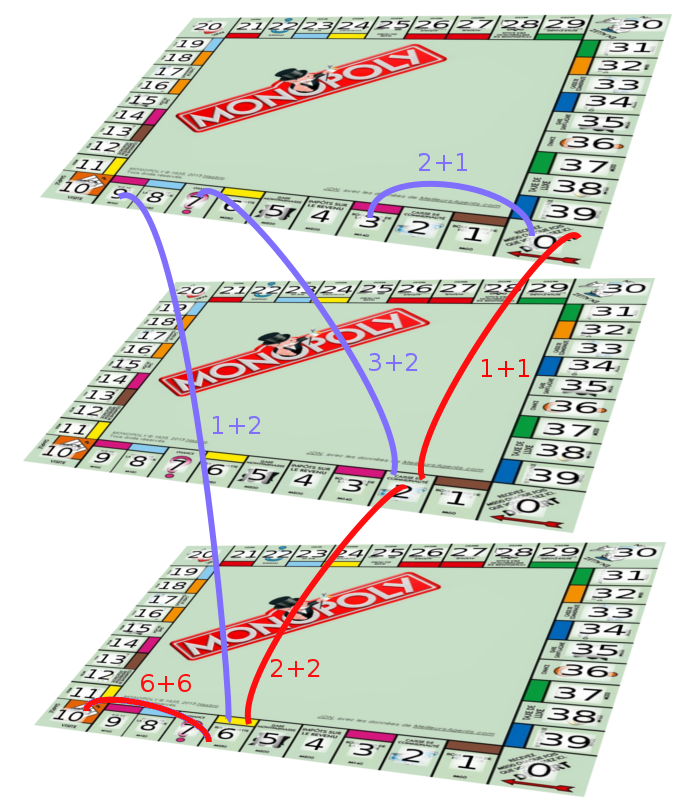
\includegraphics[scale=0.4]{./Images/MonopolyVertical.png}
	\caption{Déplacement en cas de double}
	\label{representation_double}
    \end{figure}
    
    
  \subsection{Case prison}
    \label{case_prison}
    Les règles du Monopoly stipulent que l'on peut sortir de prison de plusieurs manières 
    différentes: soit via une carte chance, soit en payant, soit en faisant un double.
    Seule les deux dernières solutions seront utilisé dans cette modélisation.  En effet,
    avoir une carte chance ne dépend pas uniquement de l'état précédent et ne peut donc
    pas être représenté facilement avec les chaînes de Markov. Les règles indiquent 
    également que l'on ne peut rester que 3 tours maximum avant d'être obligé de payer.
    Afin de représenter ces différentes cas, la case prison sera ``triplée``.  On aura
    donc trois représentations de la case prison: au premier, second et troisième tour.
    La case ''aller en prison`` sera donc considérée comme une case prison de niveau 0 et
    n'aura qu'une seule arrête visant la case ''prison premier tour``.
    Afin d'être le plus précis possible, on va calculer la probabilité de faire un double.
    Comme vu dans la \fullref{repart_des}, il y a 36 cas possible lorsque l'on lance 
    2 dés à 6 faces.  On sait qu'il y a 6 doubles.  On a donc 6 chance sur 36 de faire un
    double et chaque double: $2$, $4$, $6$, $8$, $10$ et $12$ ont chacun une chance sur 36
    d'apparaitre.  Si on ne fait pas de double (dans 5 cas sur 6), on doit relancer les 
    dés (et donc avant ça, passer à la case prison ''suivante``).
    Chaque case ''prison`` (les 3 cases cités ci-dessus) auront donc 8 arrêtes différentes:
    \begin{itemize}
     \item Payer et sortir de prison;
     \item Faire un double (et avancer du résultat de ce double), il y a donc 6 choix possibles;
     \item Ne pas réussir à faire un double (et continuer attendre).
    \end{itemize}
    
  \subsection{Case ''Chance``}
    Les cases chances peuvent faire gagner de l'argent mais également déplacé les pions 
    présent sur le plateau de jeu.  C'est évidemment ce second comportement qui sera
    étudier ici.  Le Monopoly comporte 16 cartes chances ayant la répartition suivante:
    \begin{itemize}
     \item 8 cartes faisant référence à des payements;
     \item une carte ''sortir de prison``;
     \item 7 cartes faisant référence à un déplacement.
    \end{itemize}
    On peut donc en déduire que lorsqu'un joueur pioche une carte chance, il aura une 
    7 chance sur 16 de devoir déplacer son pion.  Ces déplacements sont les suivants:
    \begin{itemize}
     \item Reculer de 3 cases;
     \item Se rendre à la case départ;
     \item Aller en prison;
     \item Se rendre à la 11ème case (où 0 est le départ);
     \item Se rendre à la 15ème case;
     \item Se rendre à la 24ème case;
     \item Se rendre à la 36ème case (dernière case avant l'arrivée).
    \end{itemize}
    Dans les 9 autres cas on lancera simplement les dés.  Les cases chances ont donc 
    beaucoup d'arrêtes.
    
  \subsection{Case ''Caisse de communauté``}
    Les cartes ''Caisse de communauté`` sont plus axé sur l'aspect financier du jeu.
    Cependant 3 cartes provoques également des déplacements des pions.
    \begin{itemize}
     \item Se rendre à la case départ;
     \item Aller en prison;
     \item Se rendre sur le première case.
    \end{itemize}
    La modélisation des cartes ''caisse de communauté`` se fait de la même manière que 
    les cartes ''Chance``.
    
  \subsection{Calcul de l'état stationnaire}
    Comme vu dans le point \ref{etat_stationnaire}, il est possible de calculer
    la distribution stationnaire de chaque case du Monopoly.  Pour se faire, on va
    se basé sur une des méthodes décrite dans ce même point, à savoir simplifier la
    fonction de base:
    \begin{align*}
     wP &= w\\
     wP &= wI\\
     w(P-I) &= 0
    \end{align*}
    Où $w$ est le vecteur stationnaire que l'on cherche, $P$ est la matrice de 
    déplacement et $I$ est la matrice identité.  On peut également noté cette 
    equation de la façon suivante:
    $$(P-I)^{T} w^{T} = 0$$
    Qui sera plus simple à implémenté dans un langage informatique.\\
    On peut également rajouter une colonne de 1 permettant d'intégrer directement la 
    contrainte suivante dans l'équation:
    $$\sum\limits_{i \in w} i = 1$$
    Cette équation part du simple principe que le vecteur résultat sera la distribution 
    de probabilité de chaque état.  Il faut donc que leur somme corresponde à 1 vu 
    que l'on exprime la probabilité de se trouver sur tous les états accèssibles, il y 
    a donc 100\% de ''chance`` de se trouver sur les états présent dans le vecteur résultat 
    (plus d'informations dans le point \ref{etat_stationnaire}).
    \paragraph{Avec un exemple concret}
    Prenons la matrice de déplacement suivante:
    \begin{align*} 
      wP = w\\ 
      % === NEW LINE ===
      % > w
      \left( 
	\begin{array}{ccc}
	w_1 & w_2 & w_3
	\end{array} 
      \right) 
      % > p
      \left( 
	\begin{array}{ccc}
	1 & 0 & 1 \\
	2 & 0 & 0 \\
	0 & 1 & 3 
	\end{array} 
      \right)
      = 
      % > w
      \left( 
	\begin{array}{ccc}
	w_1 & w_2 & w_3
	\end{array} 
      \right)  
      \\
      % === NEW LINE ===
      % w 
      \left( 
	\begin{array}{c}
	w_1\\
	w_2\\
	w_3
	\end{array} 
      \right)^T
      % (
      \left(
        % P
	\left(
	\begin{array}{ccc}
	1 & 0 & 1 \\
	2 & 0 & 0 \\
	0 & 1 & 3 
	\end{array} 
	\right)
	-
	% I
	\left(
	\begin{array}{ccc}
	1 & 0 & 0 \\
	0 & 1 & 0 \\
	0 & 0 & 1 
	\end{array} 
	\right)
      % )
      \right)
      = 0
      \\ 
      % === NEW LINE ===
      % w
      \left( 
	\begin{array}{ccc}
	w_1 & w_2 & w_3
	\end{array} 
      \right)
      % (P-I)
      \left( 
	\begin{array}{ccc}
	0 & 0 & 1 \\
	2 & -1 & 0 \\
	0 & 1 & 2 
	\end{array} 
      \right) 
      = 
      % 0
      \left( 
	\begin{array}{ccc}
	0 & 0 & 0
	\end{array} 
      \right)
      \\
      % === NEW LINE ===
      % (P-I)^T
      \left( 
	\begin{array}{ccc}
	0 & 0 & 1 \\
	2 & -1 & 0 \\
	0 & 1 & 2 
	\end{array} 
      \right)^T
      % w
      \left( 
	\begin{array}{c}
	w_1\\
	w_2\\
	w_3
	\end{array} 
      \right)
      = 
      % 0
      \left( 
	\begin{array}{c}
	0\\
	0\\
	0
	\end{array} 
      \right)
    \end{align*}
    On ajoute donc la colonne de 1:
    \begin{align*}
      \left( 
	\begin{array}{cccc}
	0 & 0 & 1 & 1 \\
	2 & -1 & 0 & 1 \\
	0 & 1 & 2 & 1
	\end{array} 
      \right)^T 
      \left( 
	\begin{array}{c}
	w_1\\
	w_2\\
	w_3
	\end{array} 
      \right)
      = 
      \left( 
	\begin{array}{c}
	0\\
	0\\
	0\\
	1
	\end{array} 
      \right)
    \end{align*}
    
    
  \subsection{Choix du langage}
    Pour modéliser le Monopoly, le langage Python a été choisi.  Il permet en effet
    d'avoir accès facilement à plusieurs librairies permettant de manipuler
    facilement des données.
    
    \subsubsection{Libraires utilisées}
      Pour manipuler plus facilement des matrices et résoudre les équations linéaire,
      la librairie ''numpy`` a été utilisé.  Concernant l'interface graphique, c'est
      la librairie ''Tkinter`` qui a été sélectionnée.
    
\section{Résultat}


\section{Conclusion}
  
  
%     ===== EXEMPLE =====
%     \begin{tikzpicture}
%       % Draw the states
%       \node[state,
% 	    text=yellow,
% 	    draw=none,
% 	    fill=gray!50!black] (s) {Sunny};
%       \node[state,
% 	    right=of s,
% 	    text=blue!30!white, 
% 	    draw=none, 
% 	    fill=gray!50!black] (r) {Rainy};
% 
%       % Connect the states with arrows
%       \draw[every loop]
% 	  (s) edge[bend right] node {} (r)
% 	  (r) edge[bend right] node {} (s)
% 	  (s) edge[bend right, auto=left]  node {0.6} (r)
% 	  (r) edge[bend right, auto=right] node {0.7} (s)
% 	  (s) edge[loop above]             node {0.4} (s)
% 	  (r) edge[loop above]             node {0.3} (r);
%     \end{tikzpicture}
  

\footnotesize
\bibliographystyle{apalike}
\bibliography{Rapport}


\end{document}